%!TEX root = ../swiatlow_thesis.tex
\label{chapter:search}
\section{Motivation}

As discussed in Section~\ref{chapter:susy:status}, the state of ATLAS SUSY searches at the Run 1 is somewhat dissappointing, in the sense that gluinos have been excluded up to even 1.4 TeV in some signal models. This is providing significant pressure on the argument of naturalness of the Higgs which SUSY had attempted to solve: without light gluinos and top-partners, SUSY requires large ``accidental'' cancellations and becomes significantly less elegant. As Section~\ref{chapter:susy:r} described, one scenario which is significantly less explored is that in which $R$-parity is violated, allowing for the decay of the LSP to SM particles. 

One particularly unexplored possibility is that of $\lambda'' > 0$, i.e., the case in which the LSP decays via `UDD' couplings through off-shell squarks. Feynman diagrams of this type are displayed in Figure~\ref{fig:search:motivation:diagrams}: the final state is composed entirely of SM particles, and in particular, entirely quarks. As there is no missing energy expected in these events, existing ATLAS SUSY analyses, which require significant \met to define signal regions, will not select these events. For this reason, even rather light gluinos-- with masses as low as 600 GeV-- could reasonably be hiding within the ATLAS dataset. Final states with neutralino LSPs are particularly well motivated: all the naturalness benefits of SUSY are maintained, but at the cost of a dark matter candidate. 

%%%%%%%%%%%%%%%%%%%%%

\begin{figure}
\centering
\subfigure[6q]{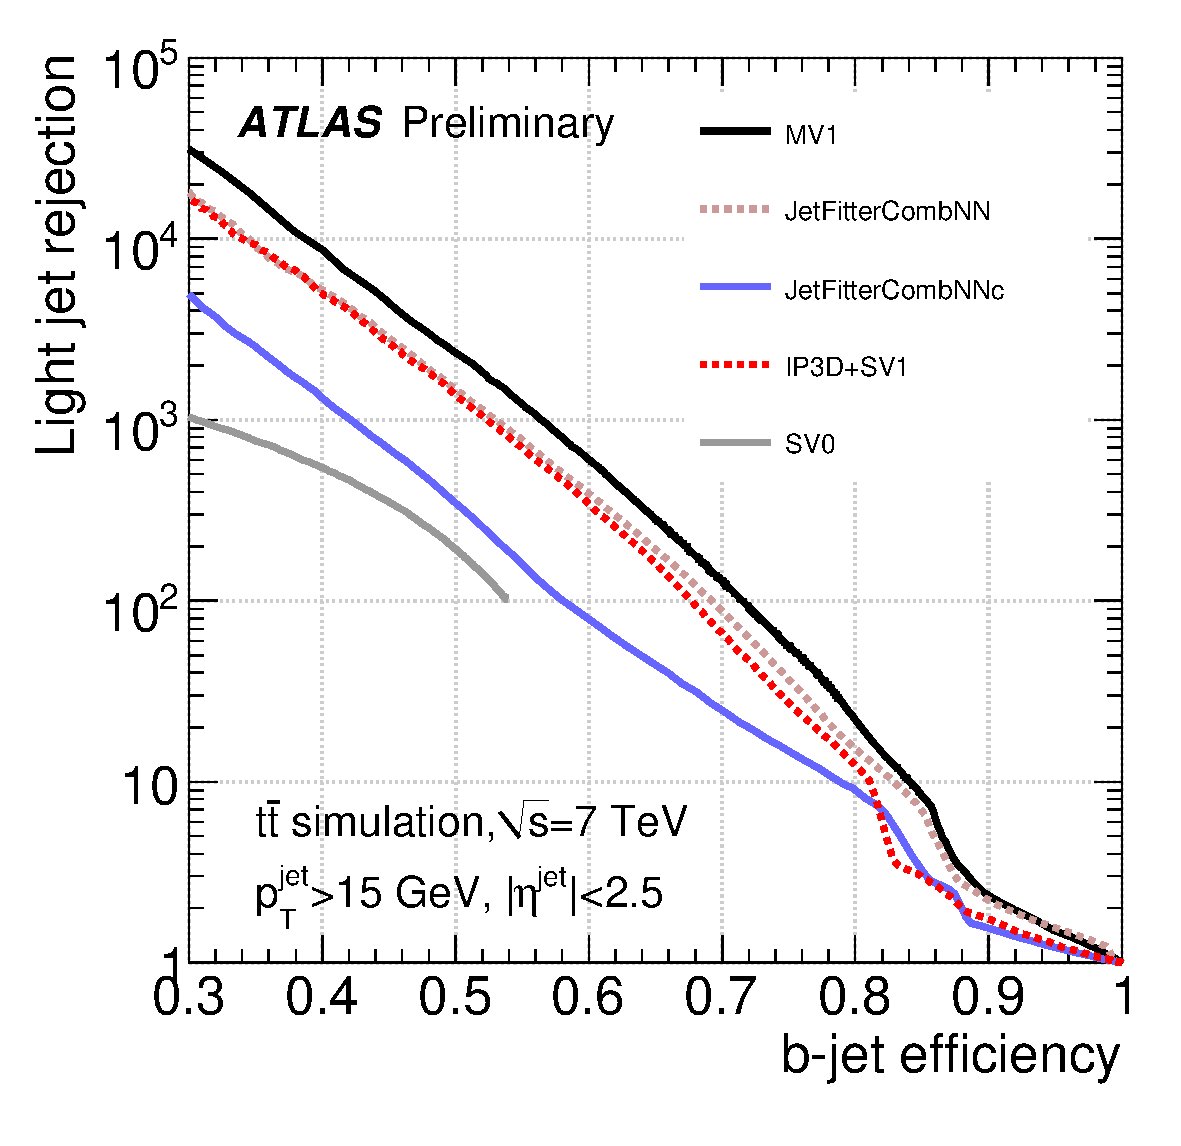
\includegraphics[width=0.45\textwidth]{mj/fig_01a.pdf}}
\subfigure[10q]{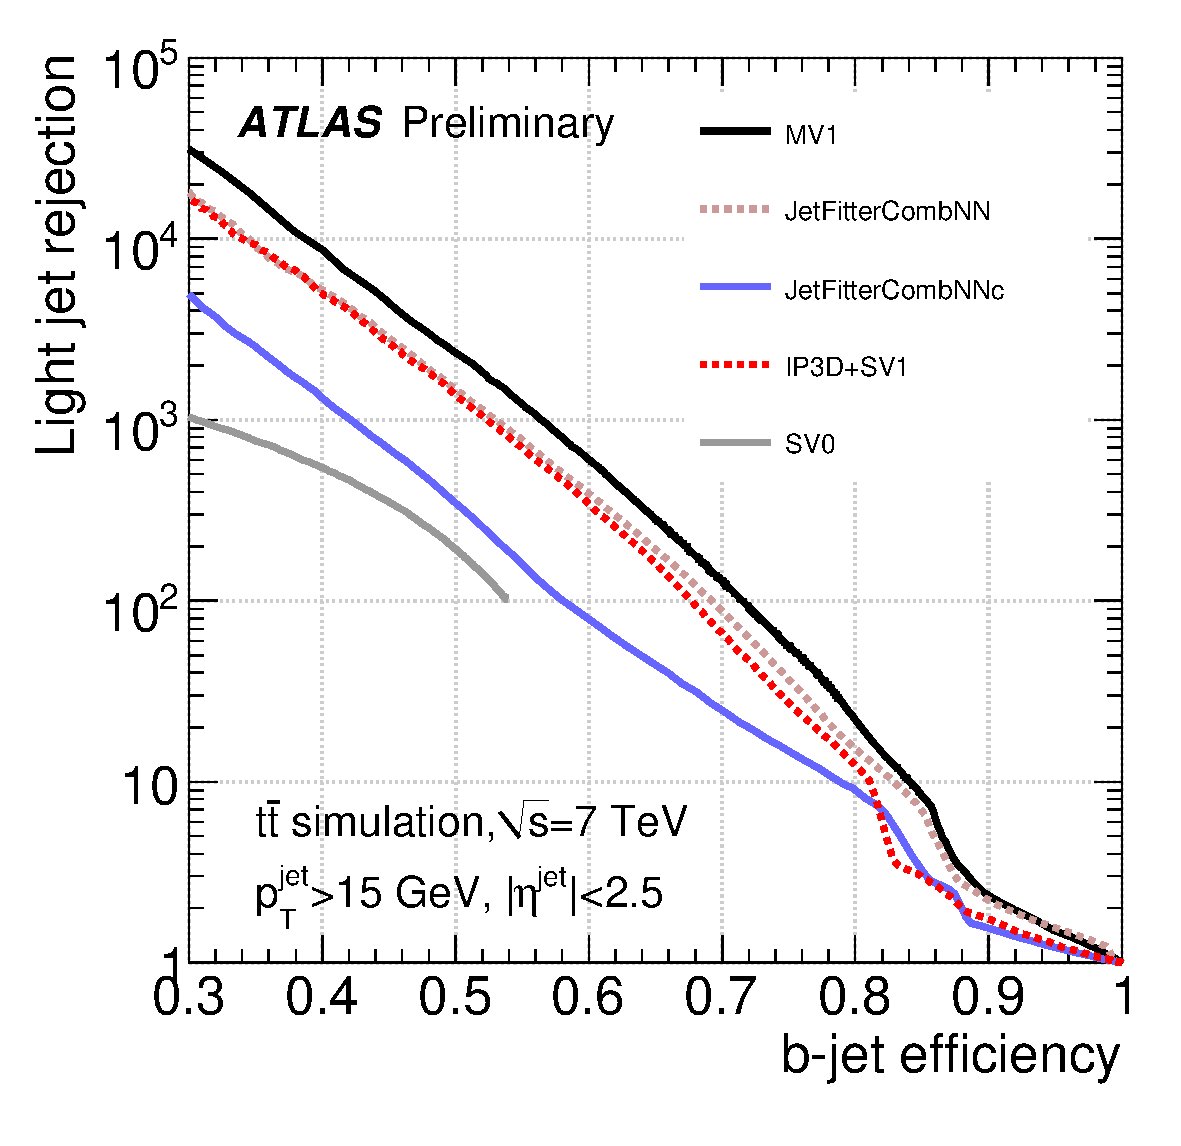
\includegraphics[width=0.45\textwidth]{mj/fig_01a.pdf}}
\label{fig:search:motivation:diagrams}
\caption{Feynman diagrams for a 6q and 10q final state with gluino pair production and RPV decays of the LSP. The 10q final state proceeds through an intermediate neutralino LSP.}
\end{figure}

%%%%%%%%%%%%%%%%%%%%%

Many different possibilities for the flavor structure of the quarks in this diagram exist. As discussed in Section~\ref{chapter:susy:r}, the  $\lambda''$ coupling is actually an anti-symmetric tensor which couples together one up type and two different down type quarks. This means, for example, that the \lsp can decay to a top-bottom-strange triplet, but not a top-bottom-bottom. The most generic assumption is to set all possibilities as equal, as a priori there is no preference for any particular combination. Moreover, there is an additional place for quark flavor to be decided, in the quarks coming from the gluino decay: these are set by the masses of the off-shell squarks in the theory. If the stop was very much lighter than the other squarks, for example, the gluinos would all decay through off-shell stops, leading to only tops from the gluino decays. Again, however, the most generic assumption is to set all squark masses to be degenerate (at 5 TeV, well above threshold), so all decays that are kinematically possible will happen. Ultimately, this means that in decay chains with many hadronically decaying top quarks can have up to 22 quarks in the final state, or as few as 10 in the case where no tops are included in the decays. 

Final states like these have largely been ignored because of the extremely difficult backgrounds: QCD multi-jet processes, which are usually suppressed by \met cuts, are dominant. The problem with QCD is actually two-fold. First, the extremely high cross-section requires very powerful variables to replace the \met cut in order to become sensitive. Additionally, the modeling of QCD backgrounds is also very challenging, generally requiring sophisticated data-driven techniques because of the inadequacy of MC simulation to model the high-multiplicity QCD final states.

An analysis searching for final states of this type is thus very attractive: SUSY could exist at rather low mass, and could be discovered if new analysis strategies and background estimation techniques were developed. Thankfully, jet substructure tools provide an answer to both elements of the problem.

%discuss final state structure, types of quarks, etc?

\section{Why Jet Substructure?}

The best way to understand the utility of jet substruture for this analysis is to consider an event display, as in Figure~\ref{fig:search:motivation:event-displays}. This display shows in the $y/\phi$ plane the \antikt $R=1.0$ Trimmed jets run on a background (left) and signal (right) event. Typically, analyses have used variables such as \Ht-- the sum of the transverse momentum of the jets-- to define a signal region. In this case, the \Ht of the two events is very similar, near $2$~TeV. However, the event on the right shows significantly more \textit{structure} in its jets than the event on the left: QCD jets are generally single-prong, while the jets in the signal have a richer topology.  

%%%%%%%%%%%%%%%%%%%%%

\begin{figure}
\centering
\subfigure[\herwigpp Dijet Background]{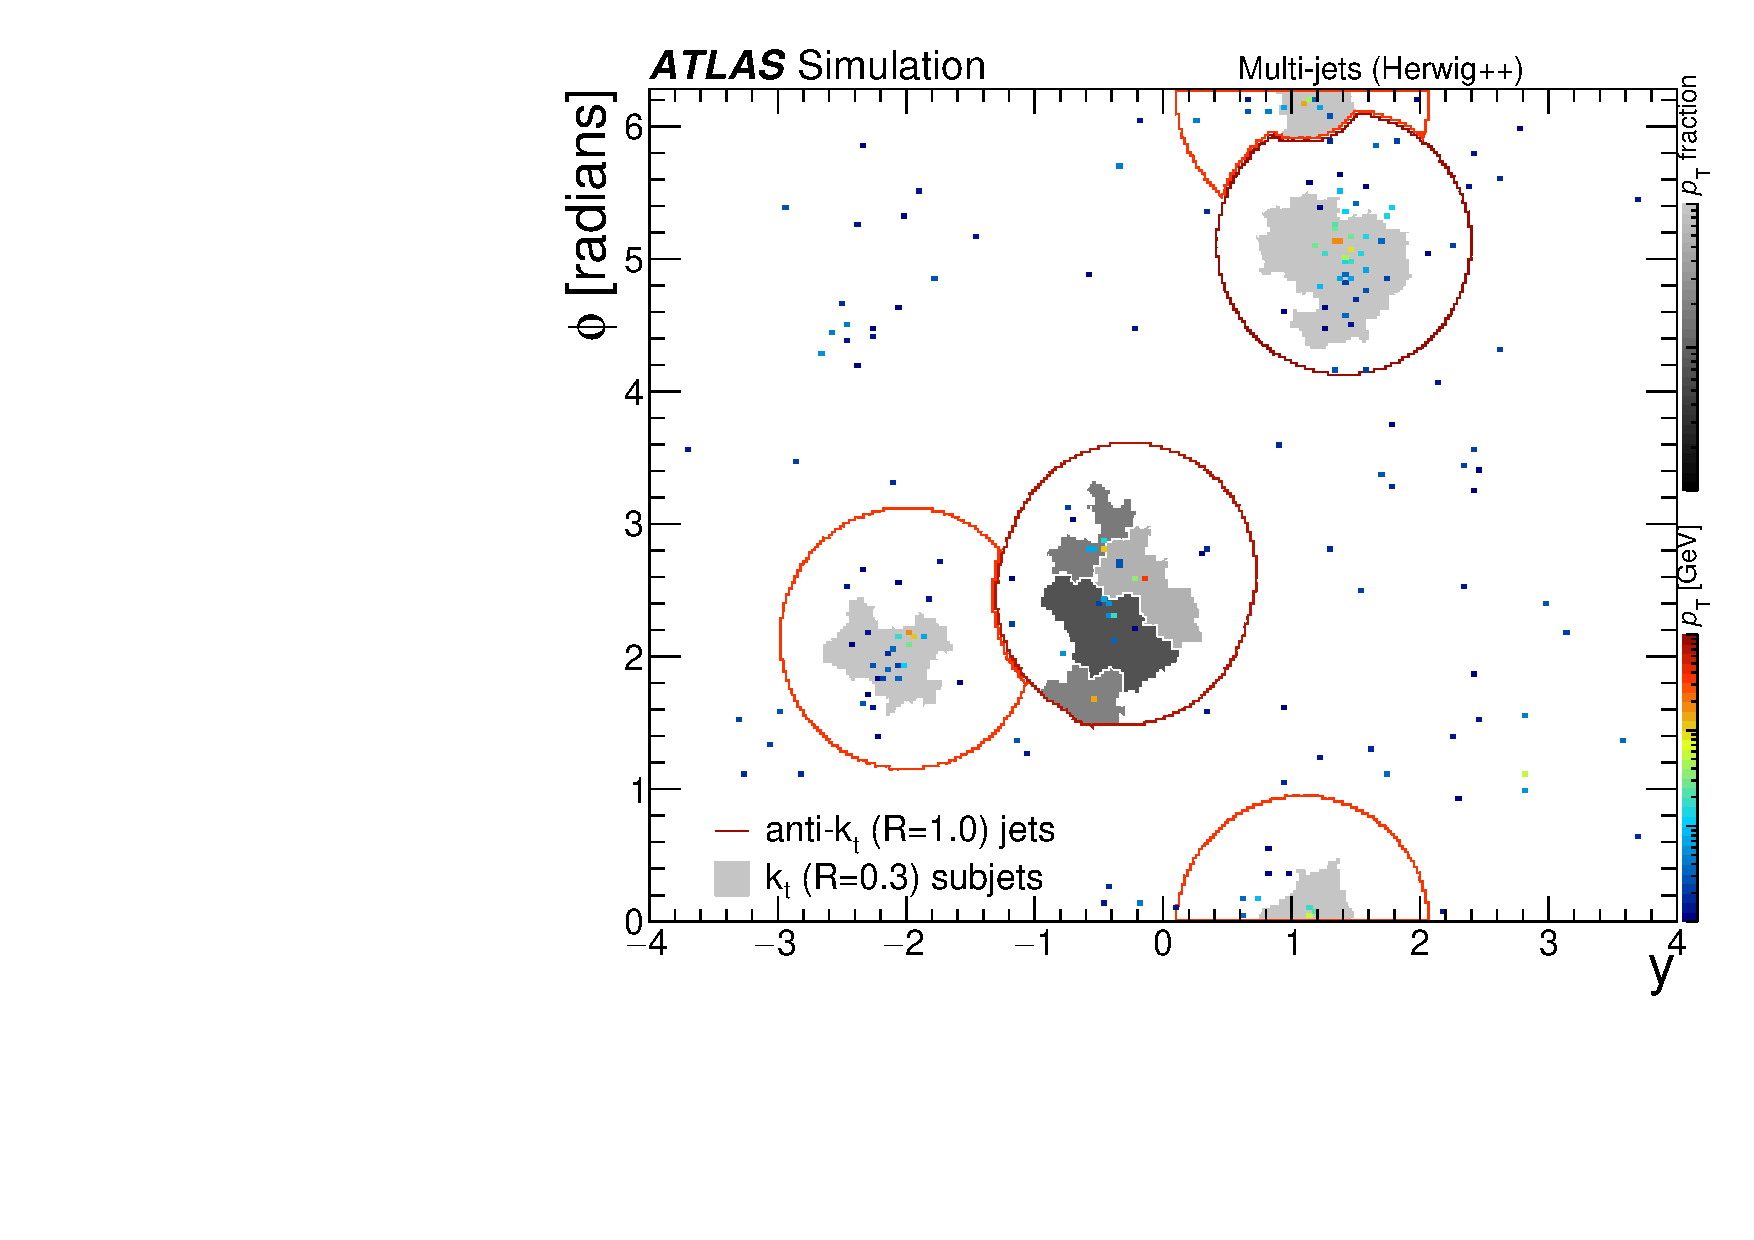
\includegraphics[width=0.45\textwidth]{mj/figaux_08f.pdf}}
\subfigure[\gl-\gl Signal]{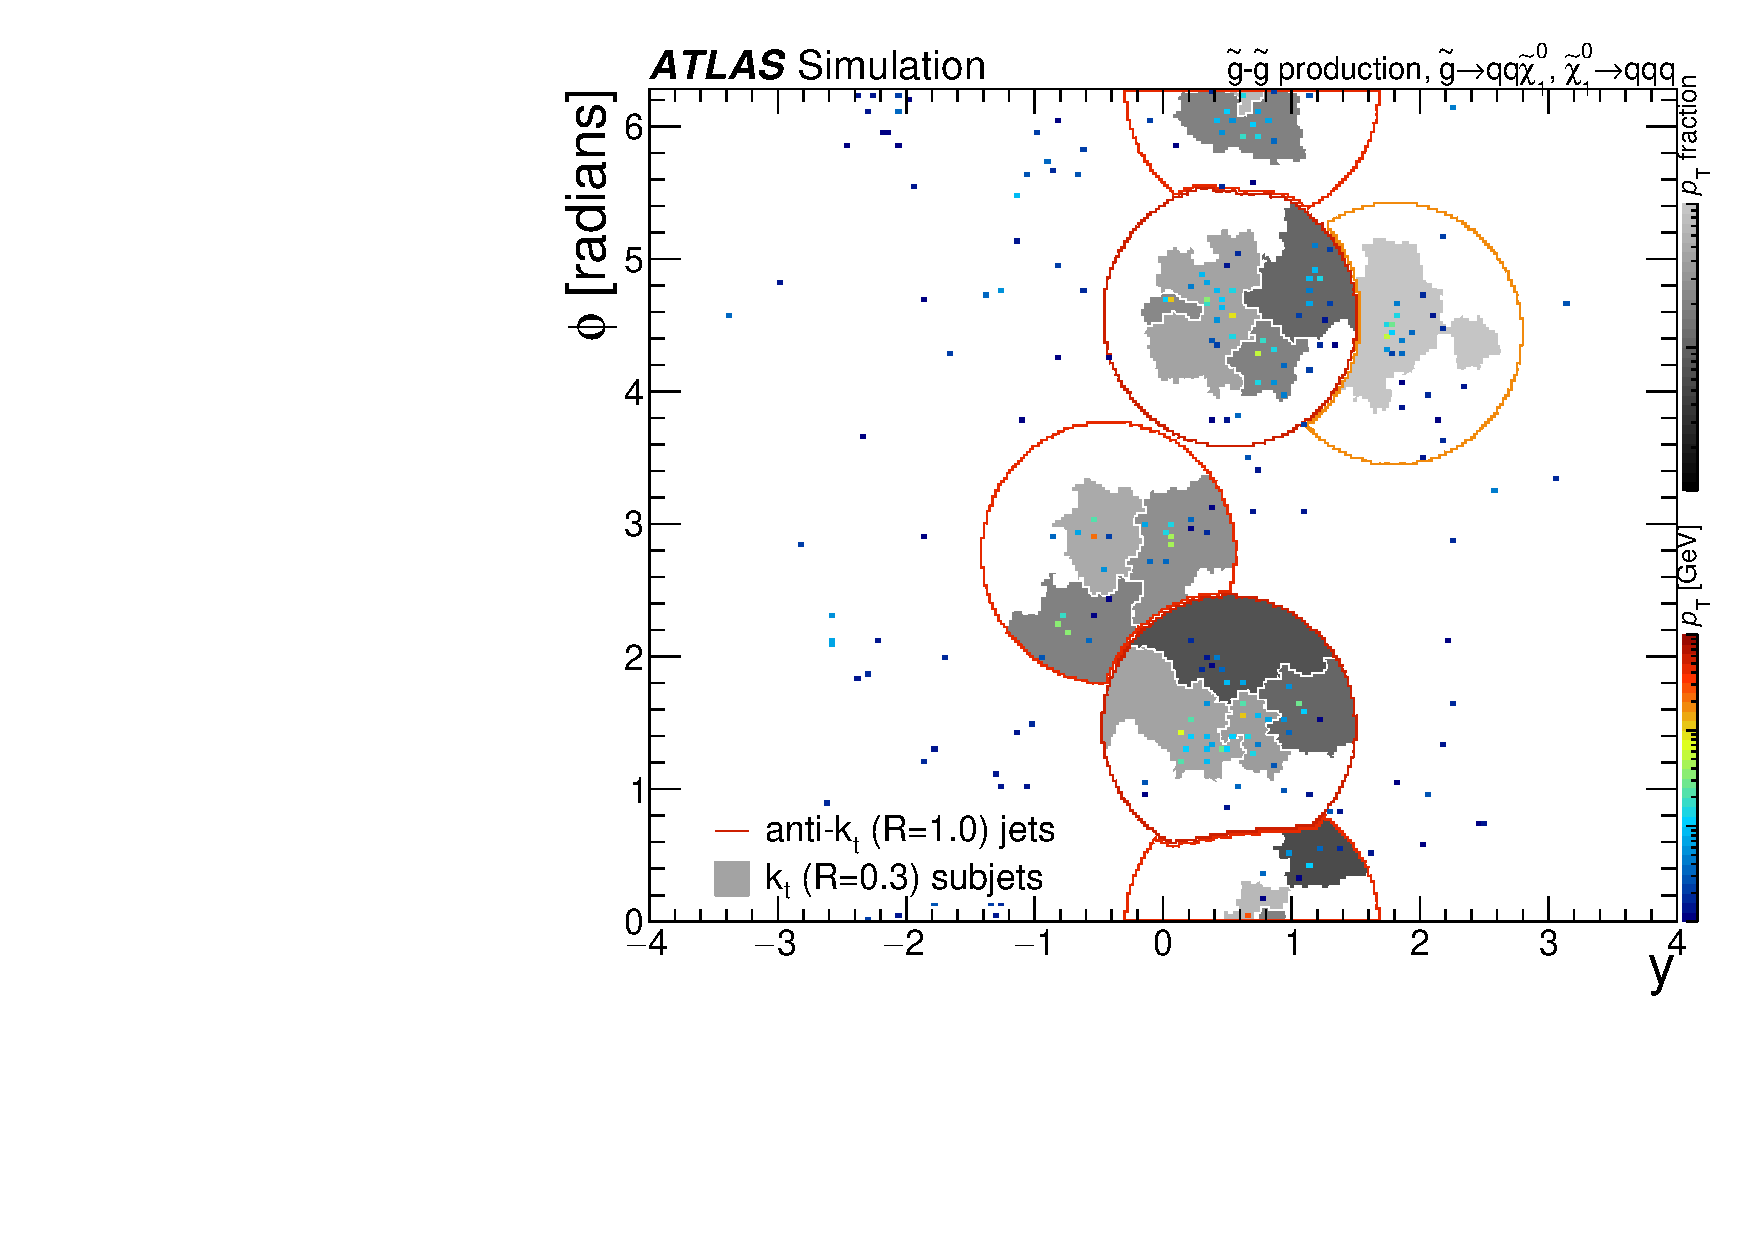
\includegraphics[width=0.45\textwidth]{mj/figaux_06f.pdf}}
\label{fig:search:motivation:event-displays}
\caption{Event displays for background and signal events with very similar \Ht (sum of jet \pt), but very different \textit{jet masses}.}
\end{figure}

%%%%%%%%%%%%%%%%%%%%%

Interestingly, these \largeR jets do not correspond to any particular top quark, or \lsp decay, or \gl decay products: the complicated, high multiplicity environment, along with relatively low \pt for quarks from the \lsp because of 3-body decays, means that most decays are not actually very collimated, and there is a great deal of overlap between quarks. All hope is not lost, however: instead of requiring mass windows, one can simply look for lots of structure. This approach is referred to as \textit{accidental substructure}: the quarks from various parts of the event accidently overlap in the \largeR jets used to reconstruct the event, and simply trying to identify ``lots of structure'' is sufficient to discriminate between signal and background. \editnote{Cite me}

Thus, jet substructure provides a path to discrimination between signal and background, which will be discussed further in Section~\ref{chapter:search:substructure:mj}. Jet substructure actually provides a path for background estimation as well: the \textit{expected structure} of QCD can be measured in control regions and extrapolated to a signal region. This strategy is discussed in Section~\ref{chapter:search:substructure:templates}. \editnote{Cite me}

\subsection{Total Jet Mass, and Other Variables}
	\label{chapter:search:substructure:mj}

A variable like \Ht (or \met) is convenient for analysis because it reduces the complexity of the event to a single scalar variable which quantifies the total energy (or missing energy) in an event. Using this approach as in inspiration, it is also possible to create variables which describe not the amount of energy, but the amount of structure in an event. \editnote{Cite me} The simplest possibility is called the \textit{Total Jet Mass}, and is defined as:
%
\begin{equation}
\MJ = \sum_{i=1}^4 M_J^i,
\end{equation}
%
where $i$ iterates over jets with some \pt and $|\eta|$ thresholds (typically 100 GeV and $2.5$ respectively, though the exact \pt cuts on the jets depend on the trigger and signal points, as described in Section~\ref{chapter:search:search}). The $\njet$ requirement is usually set to  This variable is expected to be rather sensitive to the signal: the \largeR jets in a \gl-\gl event are expected to be composed of many quarks each, and thus each have substantial mass compared to dominantly single-prong QCD backgrounds. In Figure~\ref{fig:search:motivation:event-displays}, for example, the background has $\MJ = 260$~GeV, while the signal has $\MJ = 705$~GeV: a substantial difference, even though the \HT is very similar!

There are many other similar variables which can be composed using the structure of the \largeR jets. For example, the \textit{Event-Subjettiness} is defined as:
%
\begin{equation}
T_{MN} = \left(\prod_{i=1}^4 \tau_{MN}\right)^{1/4}.
\end{equation}
%
This is the geometric mean of the n-subjettiness ratios of the leading four jets: the variable is designed to distinguish to search for compatibility of an $M$-prong structure, compared to an $N$-prong, where $M>N$. Typically $M=3$, $N=2$ and $M=2$ and $N=1$ are studied.

Another potentially useful variable is \textit{subjet counting}:
%
\begin{equation}
N_\mathrm{X}^\Sigma = \sum_{i=1}^4 N_\mathrm{X}^J,
\end{equation}
%
i.e. the total number of sub-jets (defined with some algorithm $X$) in the leading four jets in the event. The number of subjets is again expected to be strongly discriminating: for signal, it should be approximately equal to the number of quarks in the final state, and for background it should be much lower (approximately equal to one subjet per jet). 



\subsection{Jet Mass Templates}
	\label{chapter:search:substructure:templates}

\section{Constructing a Search}
\label{chapter:search:search}
	\subsection{Trigger}
	\subsection{Background Estimates}
	\subsection{Limits}
	\subsection{Future Prospects}
		...